\begin{center}
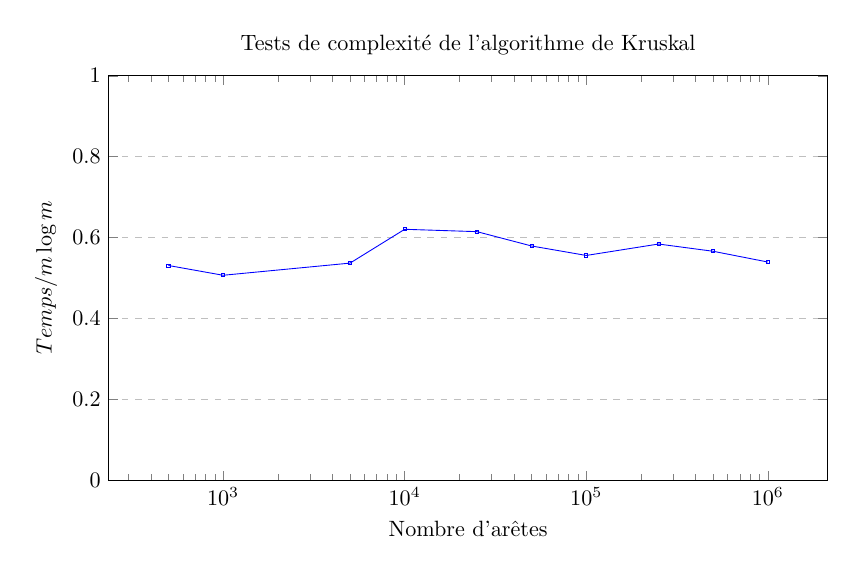
\begin{tikzpicture}[scale=0.8]
\begin{axis}[
    title={Tests de complexité de l'algorithme de Kruskal},
    xlabel={Nombre d'arêtes},
    ylabel={$Temps/m\log m$},
    ymin=0,ymax=1,
    legend pos=north west,
    ymajorgrids=true,
    grid style=dashed,
	xmode=log,
	width=13cm,
	height=8cm
]
 
\addplot[
    color=blue,
	mark=square,
	mark size=0.7
    ]
    coordinates {
		(500,0.530907263533321)(1000,0.506733826034368)(5000,0.536796418752264)(10000,0.620450563130947)(25000,0.614607869078732)(50000,0.579154914862072)(100000,0.555736629771359)(250000,0.584009143400593)(500000,0.566055578583395)(1000000,0.539472343212805)
	};
 
\end{axis}
\end{tikzpicture}
\end{center}
